\documentclass[12pt, a4paper]{article}

\usepackage[utf8]{inputenc}
% Limit the page margin to only 1 inch.
\usepackage[margin=1in]{geometry}

%Imports biblatex package
\usepackage[
backend=biber,
style=alphabetic
]{biblatex}
\addbibresource{../../algs4e.bib}

% Enables the `align' environment.
\usepackage{amsmath}
% Provides useful environments, such as:
% - \begin{proof} ...\end{proof}
\usepackage{amsthm}
\usepackage[most]{tcolorbox}

\newtheorem*{proposition}{Proposition}

% Enables using \mathbb{}, for example \mathbb{N} for the set of natural numbers.
\usepackage{amssymb}

% Allows using letters in enumerate list environment. Use, for example:
%\begin{enumerate}[label=(\alph*)]
% ...
%\end{enumerate}
\usepackage[inline]{enumitem}

% Enable importing external graphic files and provides useful commannds, like \graphicspath{}
\usepackage{graphicx}
% Images are located in a directory called images in the current directory.
\graphicspath{{./images/}}

% Make links look better by default.
% See: https://tex.stackexchange.com/questions/823/remove-ugly-borders-around-clickable-cross-references-and-hyperlinks
\usepackage[hidelinks]{hyperref}
\usepackage{xcolor}
\hypersetup{
	colorlinks,
	linkcolor={red!50!black},
	citecolor={blue!50!black},
	urlcolor={blue!80!black}
}


% Code Listings. Source:
% https://stackoverflow.com/questions/3175105/inserting-code-in-this-latex-document-with-indentation
\usepackage{listings}
\usepackage{color}

\definecolor{dkgreen}{rgb}{0,0.6,0}
\definecolor{gray}{rgb}{0.5,0.5,0.5}
\definecolor{mauve}{rgb}{0.58,0,0.82}

\lstset{frame=tb,
	language=Java,
	aboveskip=3mm,
	belowskip=3mm,
	showstringspaces=false,
	columns=flexible,
	basicstyle={\small\ttfamily},
	numbers=none,
	numberstyle=\tiny\color{gray},
	keywordstyle=\color{blue},
	commentstyle=\color{dkgreen},
	stringstyle=\color{mauve},
	breaklines=true,
	breakatwhitespace=true,
	tabsize=3
}

\newcommand{\prob}{\text{P}}
%\newcommand{\complement}{\mathsf{c}}

% Define an environment called "ex" (for Exercise) so that I can do: \begin{ex}{1.5}...\end{ex}
\newenvironment{ex}[2][Exercise]
{\par\medskip\noindent \textbf{#1 #2.}}
{\medskip}

% Define a solution environment, similar to ex (exercise) environment.
\newenvironment{sol}[1][Solution]
{\par\medskip\noindent \textbf{#1.} }
{\medskip}

\begin{document}
	\noindent Sergio E. Garcia Tapia \hfill
	
	\noindent \emph{Algorithms} by Sedgewick and Wayne (4th edition) \cite{sedgewick_wayne}\hfill
	
	\noindent January 03, 2025\hfill 
	\section*{3.4: Hash Tables}
	\begin{ex}{1}
		Insert the keys \texttt{E A S Y Q U T I O N} in that order into an initially empty
		table of $m=5$ lists, using separate chaining. Use the hash function \texttt{11 * k \% m}
		to transform the $k$th letter of the alphabet into a table index.
	\end{ex}
	\begin{sol}
		\begin{itemize}
			\item $E$ is the $5$th letter, so $11\cdot 5 \% 5 = 0$.
			\item $A$ is the $1$st letter, so $11\cdot 1 \% 5 = 1$.
			\item $S$ is the $19$th letter, so $11\cdot 19 \% 5 = 4$.
			\item $Y$ is the $25$th letter, so $11\cdot 25 \% 5 = 0$.
			\item $Q$ is the $17$th letter, so $11\cdot 17 \% e5 = 2$.
			\item $U$ is the $21$st letter, so $11\cdot 21 \% 5 = 1$.
			\item $T$ is the $20$th letter, so $11\cdot 20 \% 5 = 0$.
			\item $I$ is the $9$th letter, so $11\cdot 9 \% 5 = 4$.
			\item $O$ is the $15$th letter, so $11\cdot 15 \% 5 = 0$.
			\item $N$ is the $14$th letter, so $11\cdot 14 \% 5 = 4$.
		\end{itemize}
		See Figure~\ref{fig:ex-01}.
		\begin{figure}
			\centering
			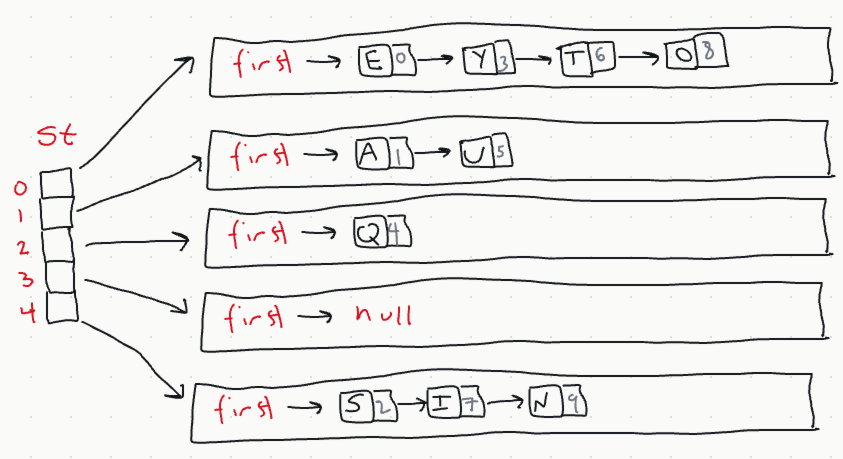
\includegraphics[width=0.7\textwidth]{exercise-01}
			\caption{Separate Chaining Hash Table from keys \texttt{E A S Y Q U T I O N}.}
			\label{fig:ex-01}
		\end{figure}
	\end{sol}
	\begin{ex}{2}
		Develop an alternate implementation of \texttt{SeparateChainingHashST} that directly
		uses the linked-list code from \texttt{SequentialSearchST}.
	\end{ex}
	\begin{sol}
		See \texttt{com.segarciat.algs4.ch3.sec4.ex02.SeparateChainingHashST}.
	\end{sol}
	\begin{ex}{3}
		Modify your implementation of the previous exercises to include an integer field for
		each key-value pair that is set to the number of entries in the table at the time
		that pair is inserted. Then implement a method that deletes all keys (and associated
		values) for which the field is greater than a given integer \texttt{k}.
		\emph{Note}: This extra functionality is useful in implementing the symbol table for
		a compiler.
	\end{ex}
	\begin{sol}
		See \texttt{com.segarciat.algs4.ch3.sec4.ex03.SeparateChainingHashST}.
	\end{sol}
	\begin{ex}{4}
		Write a program to find values of \texttt{a} and \texttt{m}, with \texttt{m} as small
		as possible, such that the hash function \texttt{(a * k) \% m} for transforming the
		$k$th letter of the alphabet into a table index produces distinct values (no collisions)
		for the keys \texttt{S E A R C H X M P L}. The result is known as a \emph{perfect hash function}.
	\end{ex}
	\begin{sol}
		See \texttt{com.segarciat.algs4.ch3.sec4.ex04.PerfectHashFunction}.
	\end{sol}
	\begin{ex}{5}
		Is the following implementation of \texttt{hashCode()} legal?
		\begin{lstlisting}
	public int hashCode()
	{ return 17; }
		\end{lstlisting}
		If so, describe the effect of using it. If not, explain why.
	\end{ex}
	\begin{sol}
		Yes, it is legal. However, because its return value is a constant expression, all
		values of this type will hash to the same index. In the case of a \texttt{SepareteChainingHashST},
		this means that all key-value pairs will belong to the same list. This will result
		in poor performance.
	\end{sol}
	\begin{ex}{6}
		Suppose that keys are binary integers. For a modular hash function with prime $m > 2$,
		prove that any two binary integers that differ in exactly one bit have different hash values.
	\end{ex}
	\begin{sol}
		\begin{proof}
			Suppose $x$ and $y$ are binary numbers that differ in exactly one bit.
			Without loss of generality, say that $x$ is larger than $y$, meaning that
			in the bit they differ, $x$ has a $1$ and $y$ has a $0$. Then $x-y$ has
			a $1$ in the bit position where $x$ and $y$ differ, and $0$s otherwise.
			Thus, $x-y$ is a power of $2$. Since $m>2$ and $m$ is prime, it follows
			that $m$ is not an even number, so $(x-y)\mod m$ is nonzero. This implies
			$x\mod m \neq y\mod m$, and hence, they both hash to different values.
		\end{proof}
	\end{sol}
	\begin{ex}{7}
		Consider the idea of implementing modular hashing for integer keys with the code
		\texttt{(a * k) \% m}, where \texttt{a} is an arbitrary fixed prime. Does this change
		mix up the bits sufficiently well that you can use nonprime \texttt{m}?
	\end{ex}
	\begin{sol}
		No. The mapping $k\mapsto a\cdot k$ is one-to-one so this variation simply re-arranges
		the inputs to the modular hashing function, but otherwise, it is equivalent to
		the modular hashing function \texttt{n \% m}, where this time $n=a\cdot k$. As
		we have discussed, this requires a prime $m$ for a reasonable spread.
	\end{sol}
	\begin{ex}{8}
		How many empty lists do you expect to see when you insert $n$ keys into a hash table
		with \texttt{SeparateChainingHashST}, for $n=10, 10^2, 10^3, 10^4, 10^5$, and $10^6$?
		\emph{Hint}: See \textbf{Exercise 2.5.31}.
	\end{ex}
	\begin{sol}
		Under the uniform hashing assumption, we expect that every integer will uniformly
		and independently distribute the keys among the integers between $0$ and $m-1$.
		Since each key hashes to an integer in this interval, we can think of the $n$
		keys as $n$ integers. Given $n$ integers belonging to the interval $[0, m)$, we want
		the expected amount of distinct values, which in turn tells us the number of
		empty lists. \textbf{Exercise 2.5.31} says that we should expect this to be
		about $m\cdot (1-e^{-\alpha})$, where $\alpha=\frac{n}{m}$. To see where this
		comes from, consider my probabilistic analysis below.
		
		For each integer $k$ satisfying $0\leq k<m$, define $X_k$ to be $1$ if $k$ occurs
		at least once in the collection of $n$ integers, and $0$ otherwise. Then $X_k$
		is a Bernoulli random variable with parameter $p$, where $p$ is the probability
		that $k$ belongs to the collection. The probability that $k$ is chosen from
		a uniform distribution of $m$ integers is $\frac{1}{m}$, and the probability that
		it is not chosen is $1-\frac{1}{m}$. If we now perform $n$ independent trials
		(justified by the uniform hashing assumption), the probability that $m$
		is never chosen among the $n$ integers is $q=1-p$, and it equals
		\begin{align*}
			q=1-p=\left(1-\frac{1}{m}\right)^n
		\end{align*}
		Since $X_k$ is a Bernoulli random variable, its expectation is given by
		\begin{align*}
			E(X_k) = p= 1-\left(1-\frac{1}{m}\right)^n
		\end{align*}
		Let $X=\sum_{k=0}^{m-1}X_k$. Then $X$ is a random variable representing the number
		of distinct values in the collection. By the linearity of expectation, we have
		\begin{align*}
			E(X) &= E\left(\sum_{k=0}^{m-1}X_k\right)=\sum_{k=0}^{m-1}EX_k=\sum_{k=0}^{m-1}p=mp
		\end{align*}
		Hence, there are about $mp$ lists that are occupied, and equivalently, about $m-mp=mq$ lists
		that are empty. To see that this is consistent with \textbf{Exercise 2.5.31}, let
		$\alpha=\frac{n}{m}$. Then $\frac{\alpha}{n} = \frac{1}{m}$, so
		\begin{align*}
			\left(1-\frac{1}{m}\right)^n &= \left(1-\frac{\alpha}{n}\right)^n
		\end{align*}
		and thus
		\begin{align*}
			\lim_{n\to\infty}\left(1-\frac{1}{m}\right)^n=\lim_{n\to\infty}\left(1-\frac{\alpha}{n}\right)^n=e^{-\alpha}
		\end{align*}
		so that
		\begin{align*}
			E(X) &= mp =m\cdot \left(1 - \left(1-\frac{1}{m}\right)^n\right)\approx m\cdot \left(1-e^{-\alpha}\right)
		\end{align*}
		For this exercise, we care about $mq\approx e^{-\alpha}$.
		Now, for the different $n$ values, noting that \texttt{SeparateChainingHashST}
		uses $m=997$ by default, we find can make the following table:
		\begin{center}
			\begin{tabular}{c|cccccc}
				$n$ & $10$ & $10^2$ & $10^3$ & $10^4$ & $10^5$ & $10^6$\\
				\hline
				Empty lists & 987 & 902 & 366 & 0 & 0 & 0
			\end{tabular}
		\end{center}
	\end{sol}
	\begin{ex}{9}
		Implement an eager \texttt{delete()} method for \texttt{SeparateChainingHashST}.
	\end{ex}
	\begin{sol}
		See \texttt{com.segarciat.algs4.ch3.sec4.ex09.SeparateChainingHashST}.
	\end{sol}
	\begin{ex}{10}
		Insert the keys \texttt{E A S Y Q U T I O N} in that order into an initially empty
		table of size $m=16$ using linear probing. Use the hash function \texttt{11 * \% m}
		to transform the $k$th letter of the alphabet into a table index. Redo
		this exercise for $m=10$.
	\end{ex}
	\begin{sol}
		First we can compute the hashes. This time I will assume that $k$th letter implies
		$k$ starts at $1$, so with $m=16$, the hash values become:
		
		\begin{lstlisting}[language={}]
E: 7
A: 11
S: 1
Y: 3
Q: 11
U: 7
T: 12
I: 3
O: 5
N: 10
		\end{lstlisting}
		The table below shows the resulting hash table in the style of the text, where
		a red color indicates the newly inserted key, black indicates probes, and gray
		keys are not examined. I have shown only keys and omitted values:
		\begin{center}
			\begin{tabular}{cc|cccccccccccccccc}
				{\color{red} key} & {\color{red} hash} &
				0 & 1 & 2 & 3 & 4 & 5 & 6 & 7 & 8 & 9 & 10 & 11 & 12 & 13 & 14 & 15\\
				\hline
				
				\texttt{E} & 7 &
				{} & {} & {} & {} & {} & {} & {} & {\color{red}\texttt{E}} & {} & {} & {} & {} & {} & {} & {} & {}\\
				
				\texttt{A} & 11 &
				{} & {} & {} & {} & {} & {} & {} & {\color{gray}\texttt{E}} & {} & {} & {} & {\color{red}\texttt{A}} & {} & {} & {} & {}\\
				
				\texttt{S} & 1 &
				{} & {\color{red}\texttt{S}} & {} & {} & {} & {} & {} & {\color{gray}\texttt{E}} & {} & {} & {} & {\color{gray}\texttt{A}} & {} & {} & {} & {}\\
				
				\texttt{Y} & 3 &
				{} & {\color{gray}\texttt{S}} & {} & {\color{red}\texttt{Y}} & {} & {} & {} & {\color{gray}\texttt{E}} & {} & {} & {} & {\color{gray}\texttt{A}} & {} & {} & {} & {}\\
				
				\texttt{Q} & 11 &
				{} & {\color{gray}\texttt{S}} & {} & {\color{gray}\texttt{Y}} & {} & {} & {} & {\color{gray}\texttt{E}} & {} & {} & {} & {\color{black}\texttt{A}} & {\color{red}\texttt{Q}} & {} & {} & {}\\
				
				\texttt{U} & 7 &
				{} & {\color{gray}\texttt{S}} & {} & {\color{gray}\texttt{Y}} & {} & {} & {} & {\color{black}\texttt{E}} & {\color{red}\texttt{U}} & {} & {} & {\color{gray}\texttt{A}} & {\color{gray}\texttt{Q}} & {} & {} & {}\\
				
				\texttt{T} & 12 &
				{} & {\color{gray}\texttt{S}} & {} & {\color{gray}\texttt{Y}} & {} & {} & {} & {\color{gray}\texttt{E}} & {\color{gray}\texttt{U}} & {} & {} & {\color{gray}\texttt{A}} & {\color{black}\texttt{Q}} & {\color{red}\texttt{T}} & {} & {}\\
				
				\texttt{I} & 3 &
				{} & {\color{gray}\texttt{S}} & {} & {\color{black}\texttt{Y}} & {\color{red}\texttt{I}} & {} & {} & {\color{gray}\texttt{E}} & {\color{gray}\texttt{U}} & {} & {} & {\color{gray}\texttt{A}} & {\color{gray}\texttt{Q}} & {\color{gray}\texttt{T}} & {} & {}\\
				
				\texttt{O} & 5 &
				{} & {\color{gray}\texttt{S}} & {} & {\color{gray}\texttt{Y}} & {\color{gray}\texttt{I}} & {\color{red}\texttt{O}} & {} & {\color{gray}\texttt{E}} & {\color{gray}\texttt{U}} & {} & {} & {\color{gray}\texttt{A}} & {\color{gray}\texttt{Q}} & {\color{gray}\texttt{T}} & {} & {}\\
				
				\texttt{N} & 10 &
				{} & {\color{gray}\texttt{S}} & {} & {\color{gray}\texttt{Y}} & {\color{gray}\texttt{I}} & {\color{gray}\texttt{O}} & {} & {\color{gray}\texttt{E}} & {\color{gray}\texttt{U}} & {} & {\color{red}\texttt{N}} & {\color{gray}\texttt{A}} & {\color{gray}\texttt{Q}} & {\color{gray}\texttt{T}} & {} & {}\\
				
				{} & {} &
				{} & {\color{black}\texttt{S}} & {} & {\color{black}\texttt{Y}} & {\color{black}\texttt{I}} & {\color{black}\texttt{O}} & {} & {\color{black}\texttt{E}} & {\color{black}\texttt{U}} & {} & {\color{black}\texttt{N}} & {\color{black}\texttt{A}} & {\color{black}\texttt{Q}} & {\color{black}\texttt{T}} & {} & {}\\
			\end{tabular}
		\end{center}
		Now for $m=10$, the hash values are the following:
		\begin{lstlisting}[language={}]
E: 5
A: 1
S: 9
Y: 5
Q: 7
U: 1
T: 0
I: 9
O: 5
N: 4
		\end{lstlisting}
		The corresponding table is shown below:
		\begin{center}
			\begin{tabular}{cc|cccccccccc}
				{\color{red} key} & {\color{red} hash} &
				0 & 1 & 2 & 3 & 4 & 5 & 6 & 7 & 8 & 9 \\
				\hline
				
				\texttt{E} & 5 &
				{} & {} & {} & {} & {} & {\color{red}\texttt{E}} & {} & {} & {} & {} \\
				
				\texttt{A} & 1 &
				{} & {\color{red}\texttt{A}} & {} & {} & {} & {\color{gray}\texttt{E}} & {} & {} & {} & {} \\
				
				\texttt{S} & 9 &
				{} & {\color{gray}\texttt{A}} & {} & {} & {} & {\color{gray}\texttt{E}} & {} & {} & {} & {\color{red}\texttt{S}}\\
				
				\texttt{Y} & 5 &
				{} & {\color{gray}\texttt{A}} & {} & {} & {} & {\color{black}\texttt{E}} & {\color{red}\texttt{Y}} & {} & {} & {\color{gray}\texttt{S}} \\
				
				\texttt{Q} & 7 &
				{} & {\color{gray}\texttt{A}} & {} & {} & {} & {\color{gray}\texttt{E}} & {\color{gray}\texttt{Y}} & {\color{red}\texttt{Q}} & {} & {\color{gray}\texttt{S}}\\
				
				\texttt{U} & 1 &
				{} & {\color{black}\texttt{A}} & {\color{red}\texttt{E}} & {} & {} & {\color{gray}\texttt{E}} & {\color{gray}\texttt{Y}} & {\color{gray}\texttt{Q}} & {} & {\color{gray}\texttt{S}} \\
				
				\texttt{T} & 0 &
				{\color{red}\texttt{T}} & {\color{gray}\texttt{A}} & {\color{gray}\texttt{E}} & {} & {} & {\color{gray}\texttt{E}} & {\color{gray}\texttt{Y}} & {\color{gray}\texttt{Q}} & {} & {\color{gray}\texttt{S}} \\
				
				\texttt{I} & 9 &
				{\color{black}\texttt{T}} & {\color{black}\texttt{A}} & {\color{black}\texttt{E}} & {\color{red}\texttt{I}} & {} & {\color{gray}\texttt{E}} & {\color{gray}\texttt{Y}} & {\color{gray}\texttt{Q}} & {} & {\color{black}\texttt{S}} \\
				
				\texttt{O} & 5 &
				{\color{gray}\texttt{T}} & {\color{gray}\texttt{A}} & {\color{gray}\texttt{E}} & {\color{gray}\texttt{I}} & {} & {\color{black}\texttt{E}} & {\color{black}\texttt{Y}} & {\color{black}\texttt{Q}} & {\color{red}\texttt{O}} & {\color{gray}\texttt{S}} \\
				
				\texttt{N} & 4 &
				{\color{gray}\texttt{T}} & {\color{gray}\texttt{A}} & {\color{gray}\texttt{E}} & {\color{gray}\texttt{I}} & {\color{red}\texttt{N}} & {\color{gray}\texttt{E}} & {\color{gray}\texttt{Y}} & {\color{gray}\texttt{Q}} & {\color{gray}\texttt{O}} & {\color{gray}\texttt{S}} \\
				
				{} & {} &
				{\color{black}\texttt{T}} & {\color{black}\texttt{A}} & {\color{black}\texttt{E}} & {\color{black}\texttt{I}} & {\color{black}\texttt{N}} & {\color{black}\texttt{E}} & {\color{black}\texttt{Y}} & {\color{black}\texttt{Q}} & {\color{black}\texttt{O}} & {\color{black}\texttt{S}} \\
			\end{tabular}
		\end{center}
	\end{sol}
	\begin{ex}{11}
		Give the contents of a linear-probing hash table that results when you insert the keys
		\texttt{E A S Y Q U T I O N} in that order into an initially empty table of initial size $m=4$
		that is expanded with doubling whenever half full. Use the hash function \texttt{11 * k \% m}
		to transform the $k$th letter of the alphabet into a table index.
	\end{ex}
	\begin{sol}
		Since the table is initially empty, the first two keys \texttt{E} and \texttt{A}
		are hashed using $m=4$:
		\begin{lstlisting}[language={}]
E: 3
A: 3
		\end{lstlisting}
		Hence the table looks as follows:
		\begin{center}
			\begin{tabular}{cc|cccc}
				{\color{red} key} & {\color{red} hash} &
				0 & 1 & 2 & 3 \\
				\hline
				
				\texttt{E} & 3 &
				{} & {} & {} & {\color{red} \texttt{E}}  \\
				
				\texttt{A} & 3 &
				{\color{red}\texttt{A}} & {} & {} & {\color{black} \texttt{E}}  \\
			\end{tabular}
		\end{center}
		When we go on to insert \texttt{S}, the test \texttt{n >= m / 2} passes because
		\texttt{n} is now 2 and \texttt{m / 2} is 2, so the table size is doubled to 8.
		In the process, the previous keys \texttt{E} and \texttt{A} are rehashed,
		and then the size stays under $m/2$ in size until \texttt{Y} is inserted.
		The hash values are now as follows:
		\begin{lstlisting}[language={}]
E: 7
A: 3
S: 1
Y: 3
		\end{lstlisting}
			The table now looks as such:
		\begin{center}
			\begin{tabular}{cc|cccccccc}
				{\color{red} key} & {\color{red} hash} &
				0 & 1 & 2 & 3 & 4 & 5 & 6 & 7 \\
				\hline
				
				\texttt{E} & 7 &
				{} & {} & {} & {} & {} & {} & {} & {\color{red} \texttt{E}} \\
				
				\texttt{A} & 3 &
				{} & {} & {} & {\color{red}\texttt{A}} & {} & {} & {} & {\color{gray} \texttt{E}} \\
				
				\texttt{S} & 1 &
				{} & {\color{red}\texttt{S}} & {} & {\color{gray}\texttt{A}} & {} & {} & {} & {\color{gray} \texttt{E}} \\
				
				\texttt{Y} & 3 &
				{} & {\color{gray}\texttt{S}} & {} & {\color{black}\texttt{A}} & {\color{red}\texttt{Y}} & {} & {} & {\color{gray} \texttt{E}} \\
			\end{tabular}
		\end{center}
		Now the table size doubles to $m=16$ as we are about to insert \texttt{Q}. Thus we rehash
		all current values, and insert at least 4 more keys (to reach a size of 8) before having
		to resize again:
		\begin{lstlisting}[language={}]
			E: 7
			A: 11
			S: 1
			Y: 3
			Q: 11
			U: 7
			T: 12
			I: 3
		\end{lstlisting}
		The table now looks as follows:
		\begin{center}
			\begin{tabular}{cc|cccccccccccccccc}
				{\color{red} key} & {\color{red} hash} &
				0 & 1 & 2 & 3 & 4 & 5 & 6 & 7 & 8 & 9 & 10 & 11 & 12 & 13 & 14 & 15\\
				\hline
				
				\texttt{E} & 7 &
				{} & {} & {} & {} & {} & {} & {} & {\color{red} \texttt{E}} & {} & {} & {} & {} & {} & {} & {} & {} \\
				
				\texttt{A} & 11 &
				{} & {} & {} & {} & {} & {} & {} & {\color{gray} \texttt{E}} & {} & {} & {} & {\color{red}\texttt{A}} & {} & {} & {} & {} \\
				
				\texttt{S} & 1 &
				{} & {\color{red}\texttt{S}} & {} & {} & {} & {} & {} & {\color{gray} \texttt{E}} & {} & {} & {} & {\color{gray}\texttt{A}} & {} & {} & {} & {} \\
				
				\texttt{Y} & 3 &
				{} & {\color{gray}\texttt{S}} & {} & {\color{red}\texttt{Y}} & {} & {} & {} & {\color{gray} \texttt{E}} & {} & {} & {} & {\color{gray}\texttt{A}} & {} & {} & {} & {} \\
				
				\texttt{Q} & 11 &
				{} & {\color{gray}\texttt{S}} & {} & {\color{gray}\texttt{Y}} & {} & {} & {} & {\color{gray} \texttt{E}} & {} & {} & {} & {\color{black}\texttt{A}} & {\color{red}\texttt{Q}} & {} & {} & {} \\
				
				\texttt{U} & 7 &
				{} & {\color{gray}\texttt{S}} & {} & {\color{gray}\texttt{Y}} & {} & {} & {} & {\color{black} \texttt{E}} & {\color{red}\texttt{U}} & {} & {} & {\color{gray}\texttt{A}} & {\color{gray}\texttt{Q}} & {} & {} & {} \\
				
				\texttt{T} & 12 &
				{} & {\color{gray}\texttt{S}} & {} & {\color{gray}\texttt{Y}} & {} & {} & {} & {\color{gray} \texttt{E}} & {\color{gray}\texttt{U}} & {} & {} & {\color{gray}\texttt{A}} & {\color{black}\texttt{Q}} & {\color{red}\texttt{T}} & {} & {} \\
				
				\texttt{I} & 3 &
				{} & {\color{gray}\texttt{S}} & {} & {\color{black}\texttt{Y}} & {\color{red}\texttt{I}} & {} & {} & {\color{gray} \texttt{E}} & {\color{gray}\texttt{U}} & {} & {} & {\color{gray}\texttt{A}} & {\color{gray}\texttt{Q}} & {\color{gray}\texttt{T}} & {} & {} \\
			\end{tabular}
		\end{center}
		Currently we are at $n=8$ and $m=16$, with the keys \texttt{O} and \texttt{N} remaining.
		We must resize so that $m=32$, so rehashing and hashing the new keys yields:
		\begin{lstlisting}[language={}]
			E: 23
			A: 11
			S: 17
			Y: 19
			Q: 27
			U: 7
			T: 28
			I: 3
			O: 5
			N: 26
		\end{lstlisting}
		Now for this last resize, there are no collisions, so the location on the table for
		each key is precisely the value of the hash after modding by $m$.
	\end{sol}
	\begin{ex}{13}
		Which of the following scenarios leads to expected \emph{linear} running time for a random
		search hit in a linear-probing hash table?
		\begin{enumerate}[label=(\alph*)]
			\item All keys hash to the same index.
			\item All keys hash to different indices.
			\item All keys hash to an even-numbered index.
			\item All keys hash to different even-numbered indices.
		\end{enumerate}
	\end{ex}
	\begin{sol}
		\begin{enumerate}[label=(\alph*)]
			\item If all keys hash to the same index, then a cluster of size $n$ is created.
			Searching for a random value in that cluster takes linear time.
			\item If all keys hash to different indices, then we expect a search hit on the
			first probe.
			\item I expect this to be the same as part (a).
			\item I expect this to be the same as part (b).
		\end{enumerate}
	\end{sol}
	\begin{ex}{14}
		Answer the previous question for a search \emph{miss}, assuming that the search key
		is equally likely to hash to each table position.
	\end{ex}
	\begin{sol}
		I expect the answers to the exactly the same.
	\end{sol}
	\begin{ex}{15}
		How many compares could it take, in the worst case, to insert $n$ keys into an initially
		empty table, using linear probing with array resizing?
	\end{ex}
	\begin{sol}
		In the worst case, all keys hash to the same value. With resizing, all keys that
		are already in the table are rehashed when the table size doubles. No compares are
		necessary for the first key. When there are $k\geq 1$ keys already in the table,
		we need $k-1$ compares because the fact all keys hash to the same value implies
		a run of length $k$. Thus, the number of compares (assuming no resizing) would be:
		\begin{align*}
			1+2+\cdots+n-1=\frac{n(n-1)}{2}
		\end{align*}
		Next, we account for resizing. When the table size is $k\geq 1$, so that $k$ keys
		need to be rehashed, the number of compares is $\frac{k(k-1)}{2}$. The number of
		times the array is resized depends on the original table size and the value of $n$.
		For simplicity, assume that the initial table size is $2$, and that $n=2^b$ for some
		integer $b$. Then the table is resized when the table has $1$ item, then again when
		it has $2$ items, and so on, until it has $2^b$ items. The table size the ends
		at size $2^{b+1}$, with $n=2^b$ items in the table. Effectively, the table is resized
		$b$ times. When it resizes from $2^j$ to $2^j+1$, where $1\leq j\leq b$,
		the table has $2^{j-1}$ items to rehash, and the necessary number of compares is:
		\begin{align*}
			1 + 2 + \cdots + 2^{j-1}-1=\frac{2^{j-1}\cdot (2^{j-1}-1)}{2}=2^{j-2}\cdot (2^{j-1}-1)
			=2^{2j-3}-2^{j-2}
		\end{align*}
		Now we sum from $j=1$ to $j=b$:
		\begin{align*}
			\sum_{j=1}^{b}\left(2^{2j-3}-2^{j-2}\right)&=
			\frac{1}{8}\sum_{j=1}^{b}4^j-\frac{1}{4}\sum_{j=1}^{b}2^j\\
		\end{align*}
		The resulting expression is roughly on the same order of magnitude as $n(n-1)/2$, where $n=2^b$.
	\end{sol}
	\begin{ex}{16}
		Suppose that a linear-probing table of size $10^6$ is half full, with occupied positions
		chosen at random. Estimate the probability that all positions with indices divisible
		by $100$ are occupied.
	\end{ex}
	\begin{sol}
		Suppose a random trial consists of choosing an integer position at random from $0$ to
		$10^6-1$. Let $X_k=1$ if the $k$th multiple of $100$ less than $10^6$ is chosen 
		at least once after $n$ trials, and $0$ otherwise. Here, $n=\frac{1}{2}10^6$ because
		the table is half-full.
		Since all positions are equally likely, the probability $k$ is chosen on a given trial
		is $\frac{1}{10^6}$. The probability that it is not chosen among the $n$ values
		is $q=\left(1-\frac{1}{10^6}\right)^n$. Thus, $P(X_k=0)=q$, and $P(X_k=1)=p=1-q$.
		
		Note that that there are $10^6/100=10^4$ multiples of $100$ less than $10^6$ (including 0).
		Let $X=\sum_{k=1}^{10^4}X_k$. Since all $X_k$ are Bernoulli with the same parameter
		$p$, and since they are independent, $X$ is binomial. Therefore, the probability that all
		$10^4$ multiples are chosen is $P(X=10^4)$, which is given by
		\begin{align*}
			P(X=10^4)=\binom{10^4}{10^4}p^{10^4}(1-p)^{10^4-10^4}=
			p^{10^4}=\left(1-\left(1-\frac{1}{10^6}\right)^n\right)^{10^4}
		\end{align*}
		Let $m$ be the table size, $n$ be the number of keys occupied in the table, and
		$\alpha=\frac{n}{m}$. Then $m=10^6$, $n=\frac{1}{2}m$, and $\alpha=\frac{1}{2}$.
		We can re-write and approximate the expression above as
		\begin{align*}
			P(X=10^4)=\left(1-\left(1-\frac{\alpha}{n}\right)^n\right)^{10^4}\approx
			(1-e^{-\alpha})^{10^4}
		\end{align*}
		Here, $1-e^{-\alpha}\approx 0.39$, and raising this to the $10^4$ power is exceedingly small.
	\end{sol}
	\begin{ex}{17}
		Show the result of using the \texttt{delete()} method on page 471 to delete \texttt{C} from
		the table resulting from using \texttt{LinearProbingHashST} with our standard indexing client
		(shown on page 469).
	\end{ex}
	\begin{sol}
		The table on 469 looks as follows:
		\begin{center}
			\begin{tabular}{c|cccccccccccccccc}
				index & 0 & 1 & 2 & 3 & 4 & 5 & 6 & 7 & 8 & 9 & 10 & 11 & 12 & 13 & 14 & 15\\
				\hline
				key & P & M & {} & {} & A & C & S & H & L & {} & E & {} & {} & {} & R & X
			\end{tabular}
		\end{center}
		Here, \texttt{C} belongs to the cluster made up by \texttt{A C S H L}. When
		\texttt{delete("C")} is issued, the keys that come after it in the cluster,
		namely \texttt{S H L}, are rehashed. From the example, we know that \texttt{S}
		hashes to \texttt{6}, \texttt{H} hashes to \texttt{4}, and \texttt{L} hashes to
		\texttt{6}. This results in \texttt{S} being at the same position, then
		\texttt{H} ends at position 5 after a collision at index 4 with \texttt{A},
		and \texttt{L} ends at position 7 after a collision at index 6 with \texttt{S}:
		\begin{center}
			\begin{tabular}{c|cccccccccccccccc}
				index & 0 & 1 & 2 & 3 & 4 & 5 & 6 & 7 & 8 & 9 & 10 & 11 & 12 & 13 & 14 & 15\\
				\hline
				key & P & M & {} & {} & A & H & S & L & {} & {} & E & {} & {} & {} & R & X
			\end{tabular}
		\end{center}
	\end{sol}
	\begin{ex}{18}
		Add a constructor to \texttt{SeparateChainingHashST} that gives the client the ability
		to specify the average number of probes to be tolerated for searches. Use array resizing
		to keep the average list size less than the specified value, and use the technique described
		on page 478 to ensure that the modulus for \texttt{hash()} is prime.
	\end{ex}
	\begin{sol}
		See \texttt{com.segarciat.algs4.ch3.sec4.ex18.SeparateChainingHashST}.
	\end{sol}
	\begin{ex}{19}
		Implement \texttt{keys()} for \texttt{SeparateChainingHashST} and \texttt{LinearProbingHashST}.
	\end{ex}
	\begin{sol}
		See \texttt{com.segarciat.algs4.ch3.sec4.ex19}.
	\end{sol}
	\begin{ex}{20}
		Add a method to \texttt{LinearProbingHashST} that computes the average cost of a search hit
		in the table, assuming that each key in the table is equally likely to be sought.
	\end{ex}
	\begin{sol}
		See \texttt{com.segarciat.algs4.ch3.sec4.ex20.LinearProbingHashST}.
	\end{sol}
	\begin{ex}{21}
		Add a method to \texttt{LinearProbingHashST} that computes the average cost of a search \emph{miss}
		in the table, assuming a random hash function. \emph{Note}: You do not have to compute any hash
		functions to solve this problem.
	\end{ex}
	\begin{sol}
		See \texttt{com.segarciat.algs4.ch3.sec4.ex21.LinearProbingHashST}.
	\end{sol}
	\begin{ex}{22}
		Implement \texttt{hashCode()} for various types: \texttt{Point2D}, \texttt{Interval},
		\texttt{Interval2D}, and \texttt{Date}.
	\end{ex}
	\begin{sol}
		See \texttt{com.segarciat.algs4.ch3.sec4.ex22}.
	\end{sol}
	\begin{ex}{23}
		Consider modular hashing for string keys with \texttt{R = 256} and \texttt{m = 255}.
		Show that this is a bad choice because any permutation of letters within a string
		hashes to the same value.
	\end{ex}
	\begin{sol}
		Modular hashing would treat each characters as a base-256 integer. If $c$ is such
		a character, then a single character would be hashed as follows:
		\begin{align*}
			(R \cdot hash + c) \mod m&=(256\cdot hash + c)\mod 255&=(hash + c)\mod 255
		\end{align*}
		where the last equality follows from the fact that $256=1\mod 255$.
		In a multi-character string, each character would be weighted by a power of $R$ that
		corresponds to its position. However, because $R\mod m$ is 1, all characters
		are weighed the same. Thus, the position of characters becomes irrelevant,
		implying that order no longer places a role and hence any permutation leads
		to the same hash.
	\end{sol}
	\begin{ex}{24}
		Analyze the space usage of separate chaining, linear probing, and BSTs for
		\texttt{double} keys. Present your results in a table like the one on page 476.
	\end{ex}
	\begin{sol}
		\begin{itemize}
			\item \texttt{SeparateChainingHashST}: There are 16 bytes of object overhead,
			$4$ bytes for the reference to its \texttt{m} field, and 8 bytes for the reference
			variable \texttt{st}, and 24 bytes for the array object itself\texttt{st} (16
			bytes overhead, 4 bytes for its length field, and 4 bytes padding). With
			4 bytes of padding, we arrive at $56$ bytes. Now, there are $m$
			\texttt{SequentialSearchST} objects, each requiring 32 bytes when empty
			(see \textbf{Exercise 3.1.21}), and an $8$ byte reference to them, for
			a total of $8m$ bytes worth of references. Overall, this means $40m$ bytes.
			If there are $n$ \texttt{double} in the table (regardless
			of which \texttt{SequentialSearchST} they are in), then the extra cost is $56n$,
			because each is store in a \texttt{Node} that takes up about 48 bytes,
			plus the actual cost for the \texttt{double} themselves, which are autoboxed
			to \texttt{Double}. Overall, the overhead is about $56+40m + 56n$,
			plus the cost for the \texttt{double} themselves.
			\item \texttt{LinearProbingHashST}: There are $16$ bytes of object overhead,
			$4$ bytes for the \texttt{n} field, $4$ bytes for the \texttt{m} field,
			$8$ bytes for the reference to the \texttt{keys} array and $24$ bytes for the
			array itself thus totaling $32$ due to \texttt{keys}, and similarly for the
			\texttt{vals} array, for a total of $88$ bytes. Now, for each key-value pair,
			there are 8 bytes for a reference to a key and 8 bytes for a reference to a value.
			When the table is half-full, meaning $n=m/2$, we have $2\cdot 8n$ for the keys and
			$2\cdot 8n$ for the values (times 2 because of the reference to unoccupied entries).
			It could also be one-eight full, in which case it's $8\cdot 8n$ in both cases.
			Altogether, the cost is around $88 + 32n$ to $88+128n$. This does not account
			for the \texttt{double} values themselves, and the fact that they would be subject
			to autoboxing to \texttt{Double}.
		\end{itemize}
	\end{sol}
	\begin{ex}{25}
		\emph{Hash cache}. Modify \texttt{Transaction} on page 462 to maintain an instance
		variable \texttt{hash}, so that \texttt{hashCode()} can save the hash value
		the first time it is called for each object, and does not have to recompute it
		on subsequent calls. \emph{Note}: This idea works only for immutable types.
	\end{ex}
	\begin{sol}
		See \texttt{com.segarciat.algs4.ch3.sec4.ex25.Transaction}.
	\end{sol}
	\begin{ex}{26}
		\emph{Lazy delete for linear probing}. Add to \texttt{LinearProbingHashST} a
		\texttt{delete()} method that deletes a key-value pair by setting the value to
		\texttt{null} (but not removing the key) and later removing the pair from the
		table in \texttt{resize()}. Your primary challenge is to decide when to call
		\texttt{resize()}. \emph{Note}: You should overwrite the \texttt{null} value if
		a subsequent \texttt{put()} operations associates a new value with the key.
		Make sure that your program takes into account the number of such \emph{tombstone}
		items, as well as the number of empty positions, in making
		the decision whether to expand or contract the table.
	\end{ex}
	\begin{sol}
		See \texttt{com.segarciat.algs4.ch3.sec4.ex26.LinearProbingHashST}.
	\end{sol}
	\begin{ex}{30}
		\emph{Chi-square statistic}. Add a method to \texttt{SeparateChainingHashST} to compute the
		$\chi^2$ statistic for the hash table. With $n$ keys and table size $m$, this
		number is defined by the equation:
		
		\begin{align*}
		\chi^2 = (m/n) \cdot ((f_0 - n/m)^2 + (f_1 - n/m)^2 + \cdots + (f_{m-1} - n/m)^2)
		\end{align*}
		
		where $f_i$ is the number of keys with has value $i$. This statistic is one way of
		checking our assumption that the hash function produces random values. If so, this
		statistic obeys a $\chi^2$ distribution with $m-1$ degrees of freedom, so its mean
		is $m-1$, and its variance is $2\cdot (m-1)$.
	\end{ex}
	\begin{ex}{34}
		\emph{Hash cost}. Determine empirically the ratio of the time required for \texttt{hash()}
		to the time required for \texttt{compareTo()}, for as many commonly-used types of
		keys for which you can get meaningful results.
	\end{ex}
	\begin{sol}
		See \texttt{com.segarciat.algs4.ch3.sec4.ex34}.
	\end{sol}
	\begin{ex}{36}
		\emph{List length range}. Write a program that inserts $n$ random \texttt{int} keys into
		a hash table of size $n / 100$ using separate chaining, then finds the length
		of the shortest and longest lists, for $n=10^3,10^4,10^5,10^6$.
	\end{ex}
	\begin{sol}
		See \texttt{com.segarciat.algs4.ch3.sec4.ex36}.
	\end{sol}
	\begin{ex}{38}
		\emph{Separate-chaining distribution}. Write a program that inserts $10^5$ random non-negative
		integers less than $10^6$ into a hash table of size $10^5$ using separate chaining, and
		that plots the total cost for each $10^3$ consecutive insertions. Discuss the extent to
		which your results validate \textbf{Proposition K}.
	\end{ex}
	\begin{sol}
		See \texttt{com.segarciat.algs4.ch3.sec4.ex38}.
	\end{sol}
	\pagebreak
	\printbibliography
\end{document}